\documentclass[aspectratio=169,11pt]{beamer}

\usepackage[T1]{fontenc}
\usepackage{lmodern}
\usepackage{booktabs}
\usepackage{array}
\usepackage{algorithm}
\usepackage{algpseudocode}
\usepackage{graphicx}
\graphicspath{{../latex_assets/}{defence_assets/}}
\usepackage{tikz}
\usetikzlibrary{positioning,arrows.meta,calc,fit,backgrounds}

% Simple, standard look
\usetheme{default}
\definecolor{accent}{HTML}{1F5F5B}
\definecolor{warn}{HTML}{A8502A}
\definecolor{grey}{HTML}{5C6670}
\definecolor{soft}{HTML}{E3EFED}
\setbeamercolor{structure}{fg=accent}
\setbeamercolor{frametitle}{fg=accent}
\setbeamercolor{title}{fg=accent}
\setbeamerfont{frametitle}{series=\bfseries}
\setbeamerfont{title}{series=\bfseries,size=\LARGE}
\setbeamertemplate{navigation symbols}{}
\setbeamertemplate{footline}[frame number]
\setbeamertemplate{itemize items}[circle]
\renewcommand{\arraystretch}{1.3}
\newcolumntype{L}[1]{>{\raggedright\arraybackslash}p{#1}}
\newcolumntype{C}[1]{>{\centering\arraybackslash}p{#1}}

\newcommand{\yes}[1]{\textcolor{accent}{\textbf{#1}}}
\newcommand{\no}[1]{\textcolor{warn}{\textbf{#1}}}
\newcommand{\h}[1]{\textcolor{grey}{#1}}
\newcommand{\remark}[1]{\par\vspace{0.35cm}{\small\textcolor{grey}{#1}}}
\algrenewcommand\algorithmicrequire{\textbf{Input:}}
\algrenewcommand\algorithmicensure{\textbf{Output:}}

\title{Multi-Agent Systems for Image Analysis:\\Object and Complex Scene Detection}
\subtitle{When Can an Automatic Answer Be Trusted? Confidence, Not Disagreement, Under a Risk Promise for Historical Illustrations}
\author{Brhanu Atsbaha}
\date{Master's thesis defence\\[6pt]
\small First advisor: Prof.\ Dr.\ Thomas Mandl \quad Second advisor: Shereen Elsayed}

\begin{document}

\begin{frame}[plain]
  \titlepage
\end{frame}

\begin{frame}{Outline}
\begin{enumerate}\setlength\itemsep{7pt}
  \item The goal, the data and the question
  \item How the system works: three agents, one decision, one promise
  \item What was wrong with the first design, and what changed
  \item Results: the 5 scene classes and the 8 object classes; what is proven, and what is likely
  \item The main question: does disagreement warn us of mistakes?
  \item How much people agree, and what that means for the results
  \item What the thesis establishes, and its limits
\end{enumerate}
\end{frame}

\begin{frame}{The goal}
The Colibri archive holds \textbf{thousands of pictures} from historical children's books. Describing them by hand is too slow, so programs (agents) describe them automatically. But the programs make mistakes.
\vspace{0.3cm}
\begin{itemize}\setlength\itemsep{8pt}
  \item Two tasks: which of \textbf{5 scene classes} (or no scene), and which of \textbf{8 object classes}.
  \item For every picture the system decides: \textbf{accept the answer}, or \textbf{send it to a person}.
  \item It gives a promise in advance: of the accepted answers, \textbf{at most 5 in 100} are wrong.
  \item Main question (RQ1): does \textbf{disagreement} between the agents warn us of mistakes?\\
        Answer: \textbf{no}. The system's own \textbf{confidence} warns better.
\end{itemize}
\remark{The contribution is not a better detector; it is knowing which answers can be trusted.}
\end{frame}

\begin{frame}{The data}
\small\begin{tabular}{@{}L{4.2cm} L{8.6cm}@{}}
\toprule
\h{Set} & \h{What it is and what it is used for}\\
\midrule
Whole archive & All pictures; every model runs on all of them\\
The 300 & Pictures a person labelled object by object: the answer key for objects\\
The scene pool & 1,250 pictures with a checked scene label, from 550 books\\
\quad practice (train) & 749: the system learns its translation rules here\\
\quad calibration & 252: the risk cut-off is chosen here\\
\quad test & 249: used only to measure, never to tune\\
The scene-class set & 992 pool pictures with a known scene class (or no scene)\\
Random archive samples & 400 + 300 pictures drawn at random from the rest of the archive, labelled by me: the archive tests\\
\bottomrule
\end{tabular}
\end{frame}

\begin{frame}{Each model on the 300 hand-labelled pictures}
\begin{columns}[T]
\column{0.52\textwidth}\small
\begin{tabular}{@{}l c c@{}}
\toprule
\h{Model, 8-class mean} & \h{Ranking} & \h{AP}\\
\midrule
\textbf{Describer (LLaVA)} & \textbf{0.903} & \textbf{0.706}\\
All three combined & 0.903 & 0.704\\
Scene matcher (SigLIP) & 0.846 & 0.560\\
Retrained object finder & 0.803 & 0.550\\
Old object finder & 0.624 & --\\
\bottomrule
\end{tabular}
\column{0.44\textwidth}\small
\begin{itemize}\setlength\itemsep{6pt}
  \item \textbf{Describer:} the strongest single model, asked one yes/no question per class; the combination ties it.
  \item \textbf{Old object finder:} good for person and animal only; the retrained one is far better.
  \item Ranking = AUROC: pictures with the class above those without it.
\end{itemize}
\end{columns}
\end{frame}

\begin{frame}{The teacher's labels, and a better teacher}
\begin{columns}[T]
\column{0.5\textwidth}\small
\begin{itemize}\setlength\itemsep{6pt}
  \item Other models confirm \textbf{71--100\%} of the labels the object finder learned from.
  \item On the 3,000-picture set they confirm only person 52\%, animal 18\%, child 2\%, weapon 0\%.
  \item 19 of 20 boxes checked by hand: all well placed; two class names wrong.
  \item \textbf{126 of 128} student misses were never labelled by the teacher.
\end{itemize}
\column{0.46\textwidth}\small
\begin{tabular}{@{}l c@{}}
\toprule
\h{Box accuracy (AP50)} & \h{Score}\\
\midrule
Old student & 0.123\\
\textbf{New student} & \textbf{0.210}\\
New teacher & 0.283\\
\midrule
Unseen pictures, old / new & 0.106 / 0.196\\
\bottomrule
\end{tabular}
\end{columns}
\remark{Biggest gains on classes the old teacher never labelled: building 0.05 $\to$ 0.23, vehicle 0 $\to$ 0.23, child 0.05 $\to$ 0.13.}
\end{frame}

\begin{frame}{Does agreement clean the training labels? Not measurably.}
The new student was trained on the teacher's boxes \emph{that a second model confirmed}. Was it the better teacher or the agreement filter that helped? Three students, same teacher, same pictures:

\vspace{0.3cm}
\begin{tabular}{@{}L{5.4cm} C{1.5cm} C{1.4cm} C{1.4cm} C{1.4cm}@{}}
\toprule
\h{Training labels} & \h{Boxes} & \h{Run 1} & \h{Run 2} & \h{Mean}\\
\midrule
All teacher boxes & 37,125 & 0.230 & 0.199 & 0.214\\
Only boxes a second model confirms & 33,657 & 0.210 & 0.253 & 0.232\\
Random subset of the same size & 33,657 & 0.205 & 0.198 & 0.201\\
\bottomrule
\end{tabular}

\vspace{0.3cm}
AP50 on the 300 hand-labelled pictures. Runs differ by up to 0.04; an earlier run put the random subset first.
\remark{The gain from 0.123 comes from the better teacher. Agreement between models does not pick the better labels.}
\end{frame}

\begin{frame}{Architecture: how the agents work together}
\centering
\resizebox{!}{0.78\textheight}{%
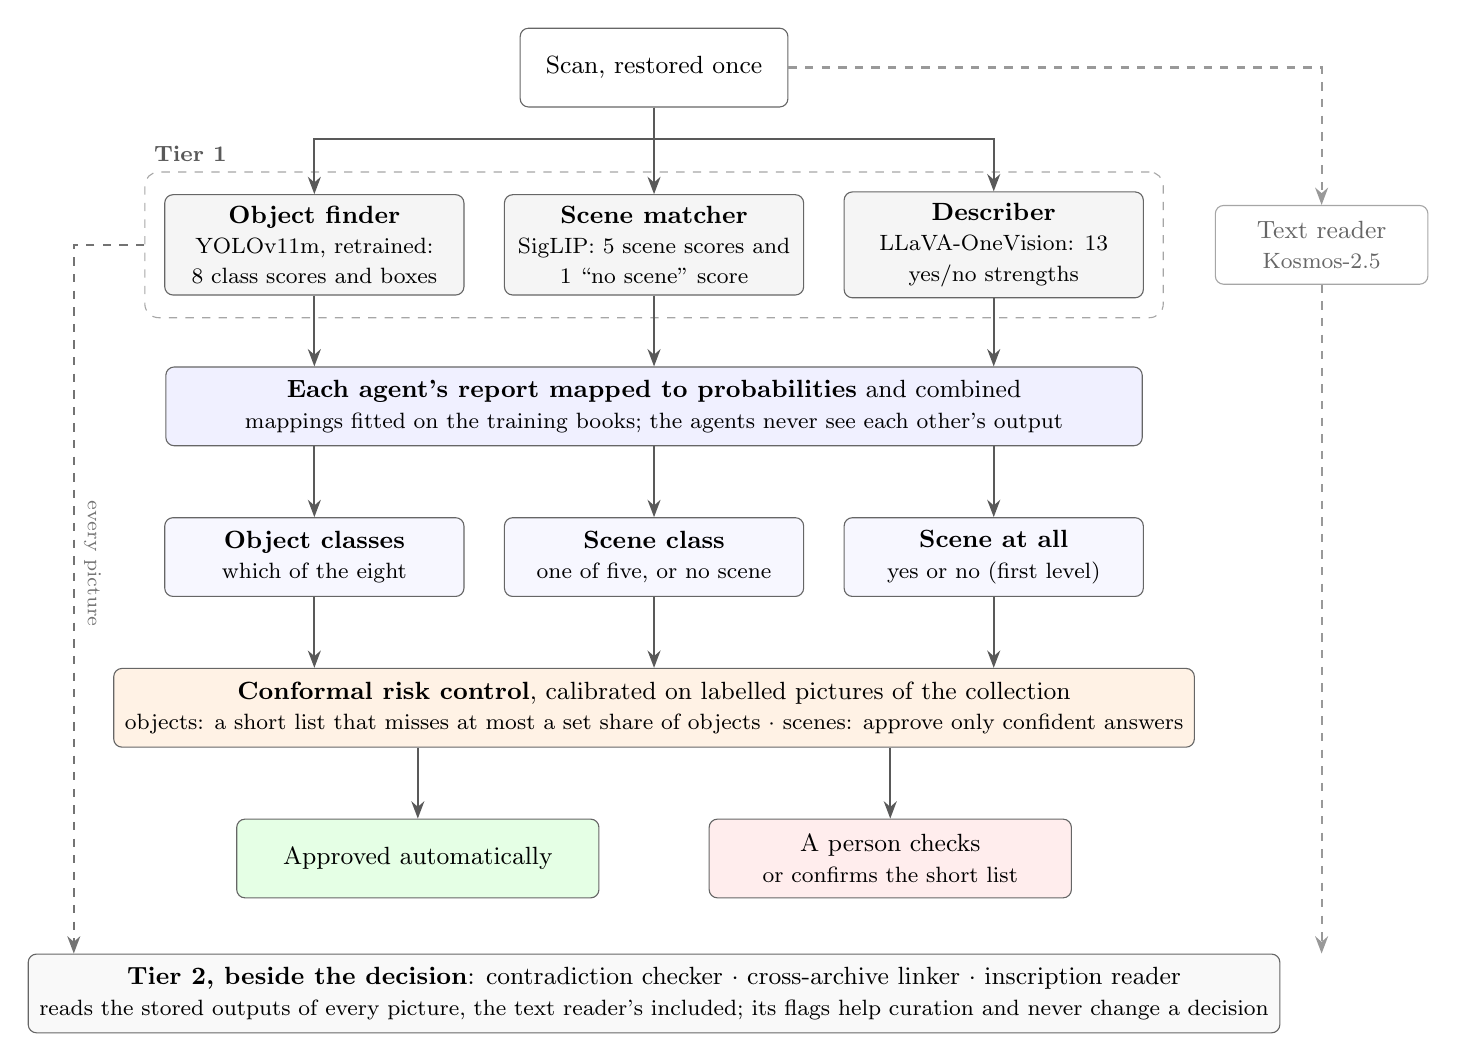
\begin{tikzpicture}[
  font=\small, >={Stealth[length=2.2mm]},
  box/.style={draw=black!60, rounded corners=3pt, align=center, inner sep=4pt, fill=white, minimum height=10mm},
  agent/.style={box, fill=gray!8, minimum width=38mm},
  mapb/.style={box, fill=blue!6, minimum width=124mm},
  outb/.style={box, fill=blue!3, minimum width=38mm},
  arr/.style={->, black!65, thick},
  tier/.style={draw=black!35, dashed, rounded corners=5pt, inner sep=7pt},
  lab/.style={font=\footnotesize\bfseries, text=black!65}]
\node[box, minimum width=34mm] (scan) {Scan, restored once};
\node[agent, below=11mm of scan] (sig) {\textbf{Scene matcher}\\{\footnotesize SigLIP: 5 scene scores and}\\{\footnotesize 1 ``no scene'' score}};
\node[agent, left=5mm of sig] (det) {\textbf{Object finder}\\{\footnotesize YOLOv11m, retrained:}\\{\footnotesize 8 class scores and boxes}};
\node[agent, right=5mm of sig] (vlm) {\textbf{Describer}\\{\footnotesize LLaVA-OneVision: 13}\\{\footnotesize yes/no strengths}};
\foreach \a in {det,sig,vlm} \draw[arr] (scan.south) -- ++(0,-4mm) -| (\a.north);
\node[box, right=9mm of vlm, minimum width=27mm, draw=black!35, text=black!60] (ocr) {Text reader\\{\footnotesize Kosmos-2.5}};
\draw[arr, black!40, dashed] (scan.east) -| (ocr.north);
\node[mapb, below=9mm of sig] (map) {\textbf{Each agent's report mapped to probabilities} and combined\\{\footnotesize mappings fitted on the training books; the agents never see each other's output}};
\foreach \a in {det,sig,vlm} \draw[arr] (\a.south) -- (\a.south |- map.north);
\node[outb, below=9mm of map.south -| det] (ob) {\textbf{Object classes}\\{\footnotesize which of the eight}};
\node[outb, below=9mm of map] (sc) {\textbf{Scene class}\\{\footnotesize one of five, or no scene}};
\node[outb, below=9mm of map.south -| vlm] (sa) {\textbf{Scene at all}\\{\footnotesize yes or no (first level)}};
\foreach \o in {ob,sc,sa} \draw[arr] (map.south -| \o.north) -- (\o.north);
\node[box, fill=orange!10, minimum width=124mm, below=9mm of sc] (crc) {\textbf{Conformal risk control}, calibrated on labelled pictures of the collection\\{\footnotesize objects: a short list that misses at most a set share of objects $\cdot$ scenes: approve only confident answers}};
\foreach \o in {ob,sc,sa} \draw[arr] (\o.south) -- (\o.south |- crc.north);
\node[box, fill=green!10, minimum width=46mm, below=9mm of crc.south, xshift=-30mm] (ok) {Approved automatically};
\node[box, fill=red!7, minimum width=46mm, below=9mm of crc.south, xshift=30mm] (per) {A person checks\\{\footnotesize or confirms the short list}};
\draw[arr] (crc.south -| ok.north) -- (ok.north);
\draw[arr] (crc.south -| per.north) -- (per.north);

\node[box, below=7mm of $(ok.south)!0.5!(per.south)$, minimum width=124mm, fill=gray!5] (t2) {\textbf{Tier 2, beside the decision}: contradiction checker $\cdot$ cross-archive linker $\cdot$ inscription reader\\{\footnotesize reads the stored outputs of every picture, the text reader's included; its flags help curation and never change a decision}};
\begin{scope}[on background layer]
\node[tier, fit=(det)(sig)(vlm), label={[lab, anchor=south west]north west:Tier 1}] (t1frame) {};
\end{scope}
\draw[arr, black!55, dashed] (t1frame.west) -- ([xshift=-5mm]t1frame.west -| crc.west) -- node[pos=0.45, above, sloped, font=\scriptsize, text=black!55]{every picture} ([xshift=-5mm]t2.north -| crc.west);
\draw[arr, black!40, dashed] (ocr.south) -- (ocr.south |- t2.north);
\end{tikzpicture}}
\remark{Three answers per picture; the risk promise decides what is approved and what a person checks.}
\end{frame}

\begin{frame}{Tier 1: three agents look at every picture}
\begin{tabular}{@{}L{2.6cm} L{6.6cm} L{3.6cm}@{}}
\toprule
\h{Agent} & \h{How it works} & \h{Output}\\
\midrule
Object finder (YOLO) & Scans the picture for boxes; per object type we keep its best box score & 8 numbers\\
Scene matcher (SigLIP) & Compares the picture with 5 scene sentences and 7 ``not a scene'' sentences (text page, sheet music, map, \dots) & 5 scene scores + 1 ``no scene''\\
Describer (LLaVA) & Asked ``Does this picture show \dots? Answer yes or no.'' per scene class and per object class; we read how strongly it leans to yes & 5 + 8 yes-strengths\\
\bottomrule
\end{tabular}
\remark{Before the agents look, every scan is restored once (Real-ESRGAN, twice the size). The text reader (Kosmos) is not used for decisions: it cannot read these old prints reliably.}
\end{frame}

\begin{frame}{Algorithm 1: deciding one picture}
\small
\begin{algorithmic}[1]
\Require picture $x$; each agent's mapping, learned on 749 training pictures; cut-offs
\Ensure a scene class, a list of object classes, and the route
\State $x \gets \textsc{Restore}(x)$; read the 3 agents \Comment{8 + 6 + 13 numbers}
\State \textbf{Scene class:} one learned mapping of all 27 numbers to chances for the 6 answers
\State \quad answer $\gets$ most likely of 6 \Comment{how much each agent counts is learned}
\State \quad if sure enough ($1 - \max P$ below the cut-off): approve, else a person
\State \textbf{Objects:} per class, mean of the 3 mapped chances
\State \quad list the classes above the threshold; a person confirms the list
\State \textbf{Scene at all} (first level): $p \gets 0.6\,p_{\text{obj}} + 0.2\,p_{\text{scene}} + 0.2\,p_{\text{vlm}}$
\State \quad scene if $p \ge 0.5$; approve if $1 - |p - 0.5|$ is below the cut-off
\end{algorithmic}
\remark{The yes/no questions are how LLaVA is read; the decision is between classes.}
\end{frame}

\begin{frame}{Algorithm 3: choosing the cut-off (conformal risk control)}
\small
\begin{algorithmic}[1]
\Require calibration pictures $i = 1..n$ ($n = 252$) with uncertainty $u_i$ and error $e_i \in \{0, 1\}$; promise $\alpha$
\For{each candidate cut-off $\lambda$ from 0.001 to 1}
  \State $\hat R(\lambda) \gets \frac{1}{n} \sum_i e_i \cdot \mathbf{1}[u_i < \lambda]$ \Comment{errors that would be approved}
\EndFor
\State $\hat\lambda \gets \max \big\{\lambda : \tfrac{n}{n+1} \hat R(\lambda) + \tfrac{1}{n+1} \le \alpha \big\}$
\State \Return $\hat\lambda$
\end{algorithmic}
\vspace{0.4cm}
\begin{itemize}\setlength\itemsep{4pt}
  \item The guarantee: on new pictures, the \textbf{average} share of wrong approved answers is at most $\alpha$.
  \item It needs no assumption about the data, only that new pictures are like the calibration ones.
  \item Example: $\alpha = 0.05$ gives $\hat\lambda = 0.829$, so a picture must be more than $0.171$ from the 0.5 line.
\end{itemize}
\remark{Source: Angelopoulos, Bates, Fisch, Lei and Schuster, \emph{Conformal Risk Control}, ICLR 2024 (arXiv:2208.02814).}
\end{frame}

\begin{frame}{Real pictures through the system}
\footnotesize
\renewcommand{\arraystretch}{0.95}\begin{tabular}{@{}L{3.3cm} L{2.6cm} L{2.2cm} L{1.7cm} L{1.8cm}@{}}
\toprule
\h{Picture (label)} & \h{Three chances} & \h{Combined} & \h{Distance from 0.5} & \h{Route}\\
\midrule
Frog (scene) & 0.94 / 0.88 / 0.89 & 0.92 scene & 0.42 & \yes{approved}\\
Soldiers with a banner (scene) & 0.98 / 0.97 / 0.98 & 0.98 scene & 0.48 & \yes{approved}\\
Frame corner (no scene) & 0.60 / 0.74 / 0.65 & 0.64 scene (wrong) & 0.14 & \no{person}\\
Leaf ornament (``drawing'') & 0.62 / 0.64 / 0.62 & 0.62 scene & 0.12 & \no{person}\\
Scroll ornament (no label) & 0.60 / 0.83 / 0.73 & 0.67 scene & 0.17 & \no{person}\\
\bottomrule
\end{tabular}

\vspace{0.2cm}
Approved only if more than \textbf{0.171} away from 0.5 (promise: 5 wrong in 100). The wrong call on the frame corner is not confident, so a person sees it.
\remark{Chances: object finder / scene matcher / describer (scene at all). Appendix A adds the scene class and object list.}
\end{frame}

\begin{frame}{Worked example: the frog}
\small
\begin{tabular}{@{}L{2.8cm} L{6.6cm} C{1.4cm} C{1.4cm}@{}}
\toprule
\h{Agent} & \h{Biggest terms} & \h{Total} & \h{Chance}\\
\midrule
Object finder & bias 0.41 $+$ animal $2.40 \times 0.954$ $-$ text $0.18 \times 0.038$ & 2.69 & \textbf{0.94}\\
Scene matcher & bias 2.01 (all its scores near 0) & 2.01 & \textbf{0.88}\\
Describer & bias 0.17 $+$ animal $2.12 \times 0.992$ $-$ text $0.35 \times 0.926$ $+ \dots$ & 2.08 & \textbf{0.89}\\
\bottomrule
\end{tabular}
\vspace{0.4cm}
\normalsize

Scene at all: $0.6 \times 0.94 + 0.2 \times 0.88 + 0.2 \times 0.89 = \mathbf{0.92}$ $\to$ scene.\\
Distance from 0.5 is 0.42, more than 0.171 $\to$ \yes{approved without a person}.\\[0.2cm]
Scene class: \textbf{drawing} 0.68 (no scene 0.29); unsure (0.32 $>$ cut-off 0.26) $\to$ a person.\\
Objects: animal 0.90, text 0.31; list at 10\%: animal, text, person, child, tree $\to$ a person confirms the list.
\end{frame}

\begin{frame}{The old design at a glance}
\centering
\resizebox{!}{0.8\textheight}{%
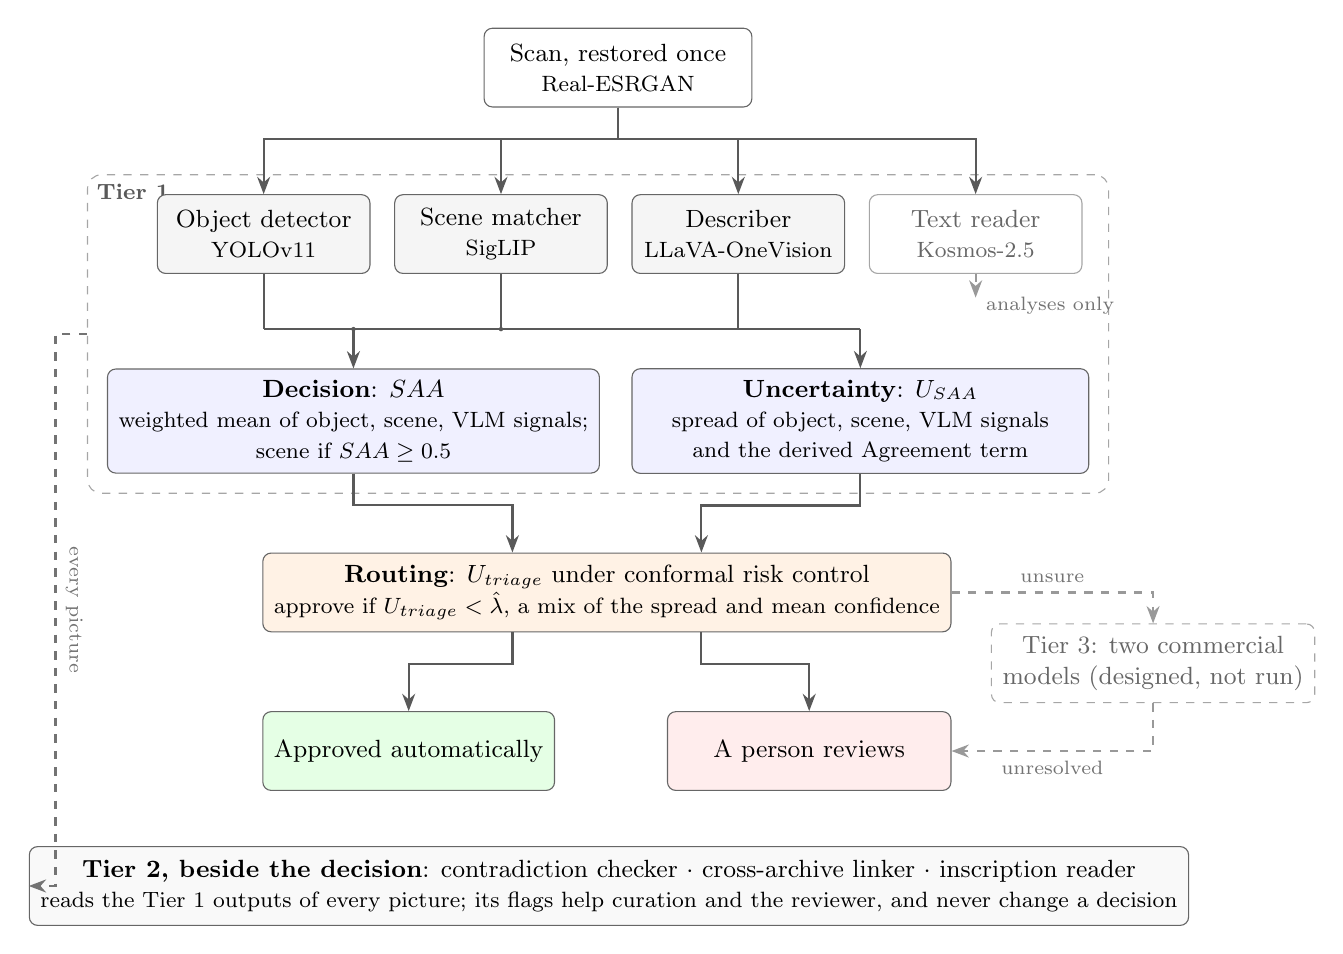
\begin{tikzpicture}[
  font=\small, >={Stealth[length=2.2mm]},
  box/.style={draw=black!60, rounded corners=3pt, align=center, inner sep=4pt, fill=white, minimum height=10mm},
  agent/.style={box, fill=gray!8, minimum width=27mm},
  calc/.style={box, fill=blue!6, minimum width=58mm},
  route/.style={box, fill=orange!10, minimum width=60mm},
  outc/.style={box, minimum width=36mm},
  tier/.style={draw=black!35, dashed, rounded corners=5pt, inner sep=7pt},
  lab/.style={font=\footnotesize\bfseries, text=black!65},
  arr/.style={->, black!65, thick}]
% row 1
\node[box, minimum width=34mm] (scan) {Scan, restored once\\{\footnotesize Real-ESRGAN}};
% row 2: Tier 1 agents
\node[agent, below=11mm of scan, xshift=-45mm] (det) {Object detector\\{\footnotesize YOLOv11}};
\node[agent, right=3mm of det] (sig) {Scene matcher\\{\footnotesize SigLIP}};
\node[agent, right=3mm of sig] (vlm) {Describer\\{\footnotesize LLaVA-OneVision}};
\node[agent, right=3mm of vlm, fill=white, draw=black!35, text=black!60] (ocr) {Text reader\\{\footnotesize Kosmos-2.5}};
\draw[arr] (scan.south) -- ++(0,-4mm) -| (det.north);
\draw[arr] (scan.south) -- ++(0,-4mm) -| (sig.north);
\draw[arr] (scan.south) -- ++(0,-4mm) -| (vlm.north);
\draw[arr] (scan.south) -- ++(0,-4mm) -| (ocr.north);
% row 3: two computations
\node[calc, below=12mm of sig.south east, anchor=north east, xshift=-1mm] (saa) {\textbf{Decision}: $SAA$\\{\footnotesize weighted mean of object, scene, VLM signals;}\\{\footnotesize scene if $SAA \ge 0.5$}};
\node[calc, right=4mm of saa] (usaa) {\textbf{Uncertainty}: $U_{\text{SAA}}$\\{\footnotesize spread of object, scene, VLM signals}\\{\footnotesize and the derived Agreement term}};
\coordinate (bus) at ($(saa.north)+(0,5mm)$);
\draw[black!65, thick] (det.south) -- (det.south |- bus);
\draw[black!65, thick] (sig.south) -- (sig.south |- bus);
\draw[black!65, thick] (vlm.south) -- (vlm.south |- bus);
\draw[black!65, thick] (det.south |- bus) -- ([xshift=0mm]vlm.south |- bus) -- (usaa.north |- bus);
\draw[arr] (saa.north |- bus) -- (saa.north);
\draw[arr] (usaa.north |- bus) -- (usaa.north);
\fill[black!65] (sig.south |- bus) circle (0.8pt) (saa.north |- bus) circle (0.8pt);
\draw[arr, black!40, dashed] (ocr.south) -- ++(0,-3mm) node[right, font=\scriptsize, text=black!55, align=left, yshift=-1mm]{analyses only};
% row 4: routing
\node[route, below=10mm of $(saa.south)!0.5!(usaa.south)$] (route) {\textbf{Routing}: $U_{\text{triage}}$ under conformal risk control\\{\footnotesize approve if $U_{\text{triage}} < \hat\lambda$, a mix of the spread and mean confidence}};
\draw[arr] (saa.south) -- ++(0,-4mm) -| ([xshift=-12mm]route.north);
\draw[arr] (usaa.south) -- ++(0,-4mm) -| ([xshift=12mm]route.north);
% row 5: outcomes
\node[outc, below=10mm of route.south west, anchor=north west, fill=green!10] (ok) {Approved automatically};
\node[outc, below=10mm of route.south east, anchor=north east, fill=red!7] (person) {A person reviews};
\draw[arr] ([xshift=-12mm]route.south) -- ++(0,-4mm) -| (ok.north);
\draw[arr] ([xshift=12mm]route.south) -- ++(0,-4mm) -| (person.north);
\node[box, above right=1mm and 5mm of person.north east, anchor=south west, draw=black!35, dashed, text=black!60, fill=white] (t3) {Tier 3: two commercial\\models (designed, not run)};
\draw[arr, black!40, dashed] (route.east) -| node[pos=0.25, above, font=\scriptsize, text=black!55]{unsure} (t3.north);
\draw[arr, black!40, dashed] (t3.south) |- node[pos=0.75, below, font=\scriptsize, text=black!55]{unresolved} (person.east);
% Tier 2
\node[box, below=7mm of $(ok.south)!0.5!(person.south)$, minimum width=96mm, fill=gray!5] (t2) {\textbf{Tier 2, beside the decision}: contradiction checker $\cdot$ cross-archive linker $\cdot$ inscription reader\\{\footnotesize reads the Tier 1 outputs of every picture; its flags help curation and the reviewer, and never change a decision}};
% tier frames
\begin{scope}[on background layer]
\node[tier, fit=(det)(sig)(vlm)(ocr)(saa)(usaa), label={[lab, anchor=north west]north west:Tier 1}] (t1frame) {};
\end{scope}
\draw[arr, black!55, dashed] (t1frame.west) -- ++(-4mm,0) |- node[pos=0.25, above, sloped, font=\scriptsize, text=black!55]{every picture} (t2.west);
\end{tikzpicture}}
\end{frame}

\begin{frame}{What was wrong with the old design}
\begin{itemize}\setlength\itemsep{9pt}
  \item The old system squeezed every picture into \textbf{four numbers}: Object, VLM, Agreement, Scene.
  \item Three of them came from \textbf{one count} by the describer:\\
        Object $=$ count$/3$; VLM $= 1$ if Object $> 0$; Agreement $= 1 - |\text{Object} - \text{VLM}|$.
  \item So only \textbf{8 different situations} were possible for the whole archive; 34\% got uncertainty exactly 0.
  \item The scene matcher was read as a forced choice: it could never say ``no scene''. Read that way it scored \textbf{0.31} on the 300 hand-labelled pictures, worse than a coin flip.
\end{itemize}
\remark{Like four witnesses where three only repeat the first one: their agreement tells you nothing new.}
\end{frame}

\begin{frame}{What we changed}
\begin{itemize}\setlength\itemsep{8pt}
  \item \textbf{Object finder:} a score for each of the 8 object types, from the retrained model.
  \item \textbf{Scene matcher:} five separate scene scores, plus one ``no scene at all'' score.
  \item \textbf{Describer:} how strongly it says ``yes'' to each scene class and each object class, instead of a rough count.
  \item \textbf{Translation:} each agent's numbers become chances: for the 6 scene answers, the 8 object classes, and a scene at all.
  \item \textbf{Routing:} by the system's confidence, not by agent disagreement; objects get a short list with a promise on missed objects.
  \item \textbf{Removed:} the derived Agreement number, and the text reader from the decision.
\end{itemize}
\end{frame}

\begin{frame}{Results: accuracy over 200 different splits}
\begin{tabular}{@{}L{4.6cm} C{3.8cm} C{3.8cm}@{}}
\toprule
\h{Measure (mean [95\% range])} & \h{Old design} & \h{Corrected design}\\
\midrule
Balanced accuracy (decision line fitted) & 0.798 & 0.815\\
Ranking quality (AUROC) & 0.829 [0.771, 0.893] & \textbf{0.866} [0.807, 0.912]\\
\bottomrule
\end{tabular}



\vspace{-0.3cm}
\remark{The corrected design calls almost every picture a scene at its 0.5 line, so its lower error rate is no gain. With a fitted line both decide equally well.}
\end{frame}

\begin{frame}{Results: pictures approved without a person}
\begin{tabular}{@{}L{3.0cm} C{2.4cm} C{2.1cm} C{2.4cm} C{2.1cm}@{}}
\toprule
 & \multicolumn{2}{c}{\h{Old design, by disagreement}} & \multicolumn{2}{c}{\h{Corrected design}}\\
\h{Promise} & \h{Approved} & \h{Real error} & \h{Approved} & \h{Real error}\\
\midrule
5 wrong in 100 & 61.1\% & 1.7\% & \textbf{76.4\%} & 5.0\%\\
10 wrong in 100 & 61.5\% & 1.9\% & \textbf{89.1\%} & 10.1\%\\
15 wrong in 100 & 70.0\% & 7.6\% & \textbf{96.8\%} & 14.0\%\\
\bottomrule
\end{tabular}

\vspace{0.2cm}
\footnotesize The old design's own triage score (0.6 disagreement + 0.4 confidence) approves 63.0\% at 5 and at 10 in 100: the corrected design still approves +13.5 and +26.1 points more.

\vspace{0.4cm}
Both designs keep every promise on average. The old one cannot use the allowed error: with only 8 possible values it is like a dimmer with 8 clicks, so it stops early and sends more pictures to a person.
\end{frame}

\begin{frame}{Same error actually delivered: the gain holds}
\begin{columns}[T]
\column{0.56\textwidth}
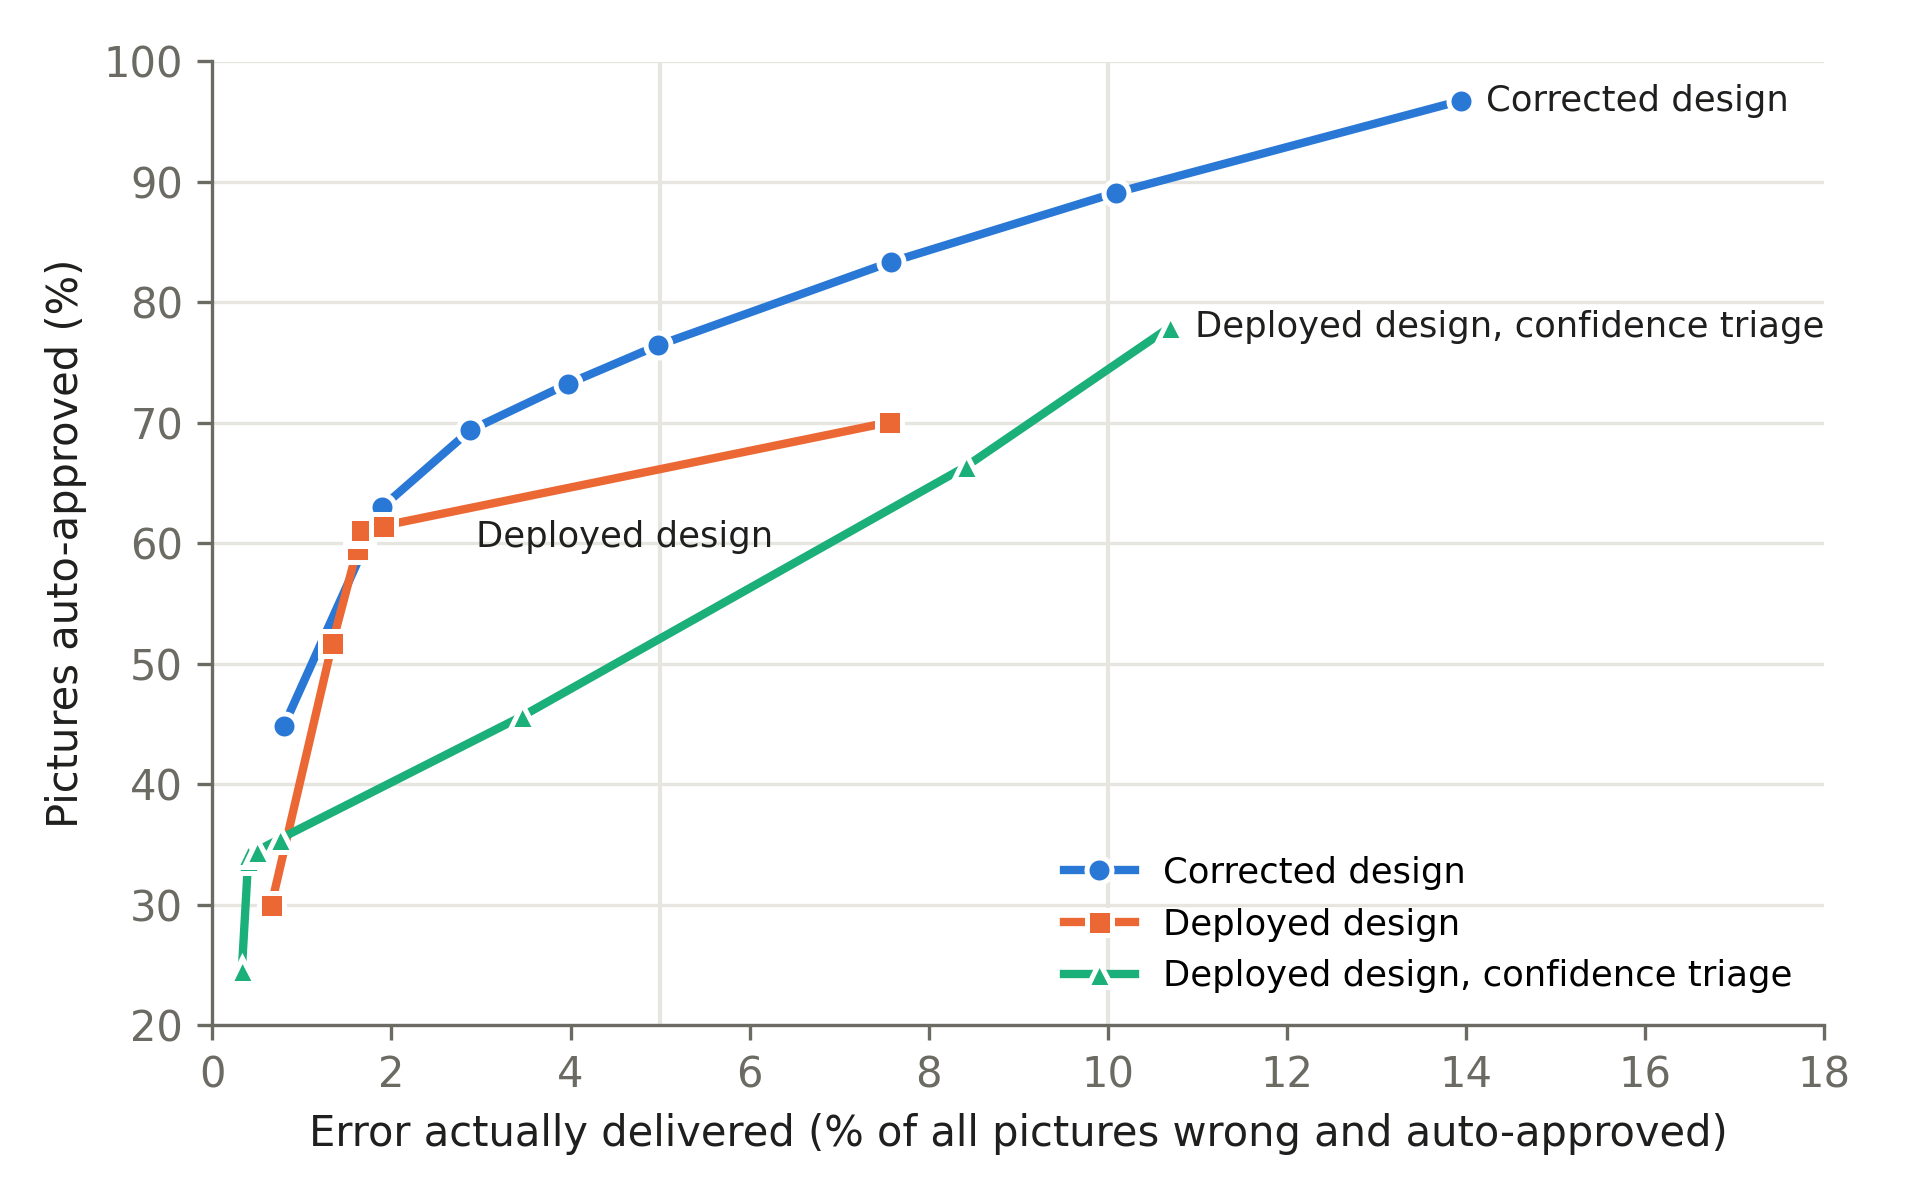
\includegraphics[width=\textwidth]{matched_risk_curve.png}
\column{0.42\textwidth}\small
The old design is safer than it promises: at a 5\% promise it delivers only 1.7\% errors, because its score takes just 8 values.

\vspace{0.25cm}
So we compare at the \textbf{same error actually delivered}:
\begin{itemize}\setlength\itemsep{3pt}
  \item at 5\%: \yes{+16.2 points}, every redraw
  \item at 10\%: \yes{+28 points}, 199 of 200 redraws
  \item at 1--3\%: +11 to +14, likely (89--97\%)
\end{itemize}
\end{columns}
\remark{200 book-disjoint redraws of 1,250 labelled pictures. The promise is met on average (0.0498 at 0.05), not on every batch.}
\end{frame}

\begin{frame}{What it saves the archive}
Review time measured from my own labelling: \textbf{3.3 s} for a scene check, \textbf{35 s} for a full annotation with boxes. For all 12,110 pictures:

\vspace{0.3cm}
\begin{tabular}{@{}L{1.8cm} C{2.5cm} C{2.7cm} C{1.9cm} C{2.6cm}@{}}
\toprule
\h{Promise} & \h{Old: still to review} & \h{Corrected: still to review} & \h{Hours saved} & \h{Wrong labels let through}\\
\midrule
5 in 100 & 4,710 & 2,853 & 18.2 h & 201 / 603\\
10 in 100 & 4,667 & 1,319 & 32.9 h & 231 / 1,222\\
15 in 100 & 3,627 & 392 & 31.8 h & 916 / 1,689\\
\bottomrule
\end{tabular}

\vspace{0.3cm}
Hours of full annotation saved by the corrected design; wrong labels as old / corrected.
\remark{The saving has a price: the corrected design uses its whole error budget. For the old error level, set the promise to 2 in 100: it still approves 63\% against 61\%.}
\end{frame}

\begin{frame}{Compared with what? The baselines}
\footnotesize
\begin{tabular}{@{}L{2.3cm} L{3.0cm} C{1.6cm} C{1.6cm} C{1.6cm} C{1.7cm}@{}}
\toprule
\h{Task} & \h{Measure} & \h{Our system} & \h{Old system} & \h{Linear probe} & \h{Zero-shot}\\
\midrule
Scene classes & balanced accuracy & 0.544 & 0.576 & 0.504 & 0.571 / 0.252\\
 & correct & 82.1\% & 77.4\% & 82.2\% & 75.7\% / 44.2\%\\
Objects & mean AUROC & \yes{0.903} & 0.624 & 0.838 & --\\
 & classes listed (10\% missed) & \yes{2.8} & -- & 4.0 & --\\
Scene or not & approved at 5\% & \yes{76.4\%} & 63.0\% & 74.0\% & --\\
\bottomrule
\end{tabular}

\vspace{0.25cm}
\begin{itemize}\setlength\itemsep{1pt}
  \item Proven: objects better than both (+0.28, +0.06 AUROC); scene-or-not +13.5 points over the old system.
  \item Not proven: better scene classes than the old system (82\% vs 77\% correct) or than one model.
\end{itemize}
\remark{Linear probe = one model's image embedding + logistic regression (standard baseline). Same pictures and 200 splits. Old system's balanced accuracy rests on 3 of 6 teaching pictures.}
\end{frame}

\begin{frame}{Results: what is proven, and what is likely}
\begin{tabular}{@{}L{5.6cm} C{2.2cm} C{2.8cm} C{1.8cm}@{}}
\toprule
\h{Corrected minus old} & \h{Mean} & \h{95\% range} & \h{Splits better}\\
\midrule
More approved at 5 in 100 & +15.3 pts & [+3.9, +29.4] & 99.5\%\\
More approved at 10 in 100 & +27.7 pts & [+15.5, +39.9] & 100\%\\
More approved at 15 in 100 & +26.7 pts & [+3.5, +44.3] & 99\%\\
\midrule
Better ranking & +0.038 & [$-0.023$, +0.098] & 88\%\\
\bottomrule
\end{tabular}

\vspace{0.4cm}
\yes{Proven:} more automatic approval at the same promise (range excludes 0).\\
\no{Likely, not proven:} better ranking (range includes 0).\\
\no{Not a gain:} the lower error rate --- at its 0.5 line the system calls almost everything a scene.
\end{frame}

\begin{frame}{Ablation: what each part adds}
\footnotesize\renewcommand{\arraystretch}{1.12}
\begin{tabular}{@{}L{3.9cm} C{1.8cm} C{1.6cm} C{2.4cm} C{2.4cm}@{}}
\toprule
\h{Version} & \h{Ranking} & \h{Wrong} & \h{Approved at 5 in 100} & \h{Worse in \% of splits}\\
\midrule
\textbf{Full system} & \textbf{0.866} & \textbf{15.6\%} & \textbf{76.4\%} & --\\
\midrule
without ``no scene'' score & 0.850 & 15.5\% & 75.3\% & 89\%\\
without object finder & 0.858 & 15.7\% & 75.8\% & 80\%\\
without scene matcher & 0.852 & 15.8\% & 75.3\% & 86\%\\
without describer & 0.867 & 15.6\% & 75.6\% & 43\%\\
\midrule
object finder alone & 0.852 & 15.8\% & 72.9\% & 84\%\\
scene matcher alone & 0.843 & 15.6\% & 72.1\% & 80\%\\
describer alone & 0.835 & 16.1\% & 74.3\% & 96\%\\
\bottomrule
\end{tabular}

\vspace{0.25cm}
\small
Removing the object finder, the scene matcher or the ``no scene'' score lowers ranking and approval a little; removing the describer changes nothing; one agent alone is always weaker. \textcolor{grey}{No single removal is proven (all 95\% ranges include 0).}
\end{frame}

\begin{frame}{Main question: does disagreement warn us of mistakes?}
\small
\begin{tabular}{@{}L{5.4cm} C{2.2cm} C{2.6cm} C{2.2cm}@{}}
\toprule
\h{Warning signal (AUROC, 0.5 = coin flip)} & \h{300 pictures} & \h{164 not in training} & \h{Test split}\\
\midrule
Per-class disagreement (tested) & \no{0.378} & 0.466 & 0.366\\
Per-class entropy & 0.286 & 0.402 & 0.252\\
Global disagreement & 0.484 & 0.458 & 0.578\\
Old disagreement signal & 0.799 & 0.646 & 0.860\\
Plain confidence & \yes{0.825} & \yes{0.728} & 0.720\\
\bottomrule
\end{tabular}

\vspace{0.3cm}
\normalsize
Difference $-0.448$ [$-0.541$, $-0.354$]: \textbf{the answer is no}.
\remark{Why: 65 of the 72 mistakes are missed scenes on pictures with few objects (0.9 classes against 1.5). There the systems' per-class scores agree most, so the mistakes sit where agreement is highest.}
\end{frame}

\begin{frame}{How much do two people agree, and the two systems?}
\begin{tabular}{@{}L{2.6cm} C{2.2cm} C{2.6cm} C{2.0cm} C{2.6cm}@{}}
\toprule
\h{Scene type} & \h{Two people ($\kappa$)} & \h{95\% range} & \h{Usable?} & \h{Two systems ($\kappa$)}\\
\midrule
landscape & 0.81 & 0.63 -- 0.94 & \yes{yes} & 0.62\\
family & 0.43 & $-0.02$ -- 0.80 & \no{barely} & 0.65\\
drawing & 0.26 & 0.13 -- 0.40 & \no{no} & 0.03\\
playing & 0.25 & 0.02 -- 0.47 & \no{no} & 0.67\\
teaching & $-0.01$ & $-0.03$ -- 0.00 & \no{no} & 0.30\\
\midrule
overall (124 pictures) & 0.34 & 0.21 -- 0.45 & & \\
\bottomrule
\end{tabular}
\remark{Same 124 pictures. Two systems = scene matcher and describer. They agree with each other more than people do for teaching, family and playing, which does not make them right. ``Drawing'' fails for both systems: almost every picture in the archive is a drawing.}
\end{frame}

\begin{frame}{The same person, two ratings: where labels diverge}
\centering
\begin{tabular}{@{}C{3.1cm} C{3.1cm} C{3.1cm} C{3.1cm}@{}}
\includegraphics[width=\linewidth,height=3.1cm,keepaspectratio]{PPN1838109994_00000266_0.jpg} &
\includegraphics[width=\linewidth,height=3.1cm,keepaspectratio]{PPN1819090841_00000469_0.jpg} &
\includegraphics[width=\linewidth,height=3.1cm,keepaspectratio]{PPN1816500674_00000210_0.jpg} &
\includegraphics[width=\linewidth,height=3.1cm,keepaspectratio]{PPN1853182958_00000082_0.jpg}\\
\small first: \textbf{drawing}\newline second: \no{none} &
\small first: \textbf{landscape}\newline second: \no{playing} &
\small first: \textbf{family}\newline second: \no{teaching} &
\small first: \textbf{landscape}\newline second: \yes{landscape}\\
\end{tabular}

\vspace{0.2cm}
\raggedright\small
143 pictures rated twice by the same person, without seeing the first label: the same scene type on \textbf{47.6\%} ($\kappa = 0.36$). 36 pictures went from ``drawing'' to ``none''.
\remark{Counting ``drawing'' as ``none'' lifts this to $\kappa = 0.58$, and agreement between two people from 0.34 to 0.50. Scene categories are interpretations, not facts.}
\end{frame}

\begin{frame}{A caution: it depends on who labels the pictures}
On 90 pictures from books the system had never seen, the old design ranked better (0.929 vs 0.894). On pictures labelled from two sources, the sources agree only moderately ($\kappa = 0.41$). So we tested on 197 pictures both had labelled:

\vspace{0.3cm}
\begin{tabular}{@{}L{6cm} C{3cm} C{3cm}@{}}
\toprule
\h{Scored with the labels of} & \h{Old design} & \h{Corrected design}\\
\midrule
the pool's labels & 0.840 & \textbf{0.865}\\
the second source & \textbf{0.818} & 0.790\\
only where both agree & 0.897 & \textbf{0.907}\\
\bottomrule
\end{tabular}

\vspace{0.3cm}
The winner changes with who decides what a scene is. We report results for our own definition.
\end{frame}

\begin{frame}{Does the promise hold on the archive? Not when calibrated on the pool}
\footnotesize 400 random archive pictures, labelled by me under one rule (people, animals, a landscape or a room = scene); test fixed before labelling.

\vspace{0.05cm}
\renewcommand{\arraystretch}{1.05}\begin{tabular}{@{}L{4.4cm} C{2.0cm} C{3.0cm} C{2.0cm}@{}}
\toprule
\h{Fitted and calibrated on the pool} & \h{Line} & \h{Approved and wrong} & \h{Approved}\\
\midrule
Labels as used so far & 0.5 & \no{16.2\%} & 78\%\\
One rule for ``scene'' & 0.5 & \no{8.5\%} & 94\%\\
\midrule
\h{Calibrated on archive pictures} & & & \\
One rule, half of the 400* & 0.5 & \yes{4.8\%} & \textbf{81\%}\\
One rule, 294 new pictures (fixed in advance) & 0.5 & 5.9\% & \textbf{80\%}\\
\quad same, promise set to 2.5\% & 0.5 & \no{4.6\%} & 64\%\\
\bottomrule
\end{tabular}

\vspace{0.02cm}
Causes: two definitions of a scene in the pool, and a pool that is not a random draw (16\% vs 38\% no scene).
\remark{* Added after the first test. New pictures: both promises narrowly missed; the two samples differ (38\% vs 47\% no scene): labels moved?}
\end{frame}

\begin{frame}{The 8 object classes: ranked well, promised as a short list}
\footnotesize 300 hand-annotated pictures. AUROC: pictures with the class ranked above those without. Right: objects kept in the list when at most 10 in 100 may be missed.

\scriptsize\renewcommand{\arraystretch}{0.95}\begin{tabular}{@{}L{1.7cm} C{1.6cm} C{1.4cm} C{1.6cm} | C{2.6cm}@{}}
\toprule
\h{Class} & \h{Object finder} & \h{LLaVA} & \h{Combined} & \h{Kept in the list}\\
\midrule
person & 0.920 & 0.938 & \textbf{0.953} & 97\%\\
child & 0.685 & \textbf{0.864} & 0.830 & 79\%\\
animal & 0.865 & \textbf{0.930} & 0.924 & 92\%\\
building & 0.826 & 0.955 & \textbf{0.960} & 79\%\\
weapon & 0.648 & 0.812 & \textbf{0.827} & 68\%\\
vehicle & 0.863 & \textbf{0.987} & 0.984 & 89\%\\
tree & 0.814 & 0.858 & \textbf{0.878} & 85\%\\
text & 0.807 & \textbf{0.880} & 0.866 & 92\%\\
\midrule
Mean & 0.803 & 0.903 & 0.903 & \yes{9.2\% per picture}\\
\bottomrule
\end{tabular}

\footnotesize Each picture gets a list of 2.8 classes; a person strikes out 1.6 wrong ones. Boxes: mean AP50 0.210.
\remark{A promise on all decisions confirms at most 0.4\% of objects. LLaVA alone is as good as the combination; learning the weights does not help here.}
\end{frame}

\begin{frame}{The 5 scene classes: shortlisted, not decided}
\footnotesize 992 pictures of the pool with a known class (no scene 486, drawing 341, landscape 76, family 51, playing 32, teaching 6); 200 splits by book.

\vspace{0.1cm}
\begin{tabular}{@{}L{4.4cm} C{1.7cm} C{1.3cm} C{1.3cm} C{1.6cm}@{}}
\toprule
 & \h{Balanced accuracy} & \h{Family found} & \h{Playing found} & \h{Landscape found}\\
\midrule
\textbf{The system} (learned) & \textbf{0.544} & 44\% & 27\% & 62\%\\
Fixed 0.6/0.2/0.2 (planned) & 0.401 & \no{13\%} & \no{11\%} & \no{25\%}\\
LLaVA alone & 0.507 & 48\% & 8\% & 61\%\\
The system, balanced* & 0.625 & 55\% & 55\% & 86\%\\
\bottomrule
\end{tabular}

\vspace{0.15cm}
\begin{itemize}\setlength\itemsep{2pt}
  \item 5\% promise: 69\% approved, nearly all \textbf{``no scene''} (1.6\% wrong) or \textbf{``drawing''} (16\% wrong); specific classes $\to$ \textbf{a person}.
  \item Short list at 10\%: right for 90.4\% (1.3 classes), but only 66\% of family, 42\% of playing; balanced*: 82\%, 80\%, 94\% (landscape).
\end{itemize}
\remark{* Added after the planned run; LLaVA alone fitted that way: 0.631. People agree on these classes only moderately ($\kappa$ = 0.34).}
\end{frame}

\begin{frame}{What the thesis establishes}
\footnotesize\renewcommand{\arraystretch}{0.88}\begin{tabular}{@{}L{2.2cm} L{11.0cm}@{}}
\toprule
\yes{Proven} & Disagreement no better than confidence (0.378 vs 0.825; per task 0.78--0.82 vs 0.83--0.84).\\
 & Scene or not, inside the pool: +13.5 points approved at a 5\% promise, +26.1 at 10\% (vs the old triage score).\\
 & Objects: a list of 2.8 classes per picture missing 9.2\% per picture, as promised at 10\% (10.8\% of all objects).\\
 & Archive, calibrated on archive pictures: just above the promised level (5.4--5.9\% at 80\% approved).\\
 & Grading against the teacher hides the failure (0.768 vs 0.146); a better teacher: 0.123 $\to$ 0.210.\\
 & Scene classes: learning the combination beats the fixed weights (0.401 $\to$ 0.544).\\
\midrule
\textbf{Likely} & Better ranking (0.829 $\to$ 0.866; corrected $t$-test only).\\
\midrule
\no{Not shown} & Better scene / no-scene decisions (0.815 vs 0.798 balanced accuracy).\\
 & A pool-calibrated cut-off keeping its promise on the archive (16.2\% wrong).\\
 & Objects confirmed without a person.\\
 & A specific scene class given automatically (only ``no scene'', ``drawing'').\\
 & Three agents clearly beating one (learned: only slightly ahead of LLaVA).\\
 & Ranking gain under another labeller; agreement picking better training labels.\\
\bottomrule
\end{tabular}
\remark{Not a better detector: a tested account of when an automatic answer can be trusted.}
\end{frame}

\begin{frame}{Limits and future work}
\begin{columns}[T]
\column{0.48\textwidth}
\textbf{Limits}
\begin{itemize}\setlength\itemsep{2pt}
  \item Where all agents are wrong together, nothing warns: mistakes are 6 times more frequent on the sparsest pictures.
  \item The promise holds on average, and only for pictures like the calibration pictures: calibrate on a random sample of the collection.
  \item The archive test rests on one person's labels (13 of 17 repeats the same).
  \item 249 test pictures; the class teaching has only 6 labelled pictures.
  \item Tier 3 is designed, not run.
\end{itemize}
\column{0.48\textwidth}
\textbf{Future work}
\begin{itemize}\setlength\itemsep{2pt}
  \item A second rater on the 400 random archive pictures.
  \item A model trained on archive drawings for the shared blind spot.
  \item The same design on a second archive.
  \item Scene classes learned on archive pictures (on the archive the pool's mapping reaches 0.351, not 0.544); a promise per scene class (needs more rare-class labels).
\end{itemize}
\end{columns}
\end{frame}

\begin{frame}
\centering
\vspace{1.2cm}
{\Large\textbf{\textcolor{accent}{Thank you}}}

\vspace{0.6cm}
Questions and discussion
\end{frame}

\begin{frame}
\centering
\vspace{1.4cm}
{\large\textcolor{grey}{Backup slides}}
\end{frame}

\begin{frame}{Step 1: a picture arrives}
\begin{columns}[T]
\column{0.53\textwidth}
\begin{enumerate}\setlength\itemsep{8pt}
  \item A scanned picture arrives.\\ \textcolor{grey}{Example: page 48 of book PPN1780419686, a coloured drawing of a frog, named in four languages.}
  \item It is \textbf{cleaned once}: sharpened and made twice as large (Real-ESRGAN).
  \item The same clean picture goes to \textbf{all three agents at the same time}. Each works alone and never sees the others' answers.
  \item Each agent gives back a short list of numbers, each between 0 and 1.
\end{enumerate}
\column{0.42\textwidth}\footnotesize
\begin{tabular}{@{}l c L{2.1cm}@{}}
\toprule
\h{Agent} & \h{Count} & \h{What}\\
\midrule
Object finder & \textbf{8} & one per object type\\
Scene matcher & \textbf{6} & 5 scenes + ``no scene''\\
Describer & \textbf{13} & one per scene class and per object type\\
\bottomrule
\end{tabular}
\end{columns}
\remark{The 8 object types: person, child, animal, building, weapon, vehicle, tree, text. The 5 scenes: teaching, family, playing, landscape, drawing.}
\end{frame}

\begin{frame}{Object finder: from the picture to 8 numbers}
\begin{enumerate}\setlength\itemsep{5pt}
  \item The picture is resized to 640 pixels.
  \item The finder looks at many places and sizes at once and asks: \emph{is there a thing here, and which of my 8 types is it?}
  \item Each thing it finds gets a \textbf{box} with a type and a score from 0 (unsure) to 1 (very sure).
  \item For each type we keep the score of its \textbf{best box}. No box of that type $\to$ 0.
\end{enumerate}
\vspace{0.3cm}
\footnotesize
\begin{tabular}{@{}l *{8}{C{1.1cm}}@{}}
\toprule
 & \h{person} & \h{child} & \h{animal} & \h{building} & \h{weapon} & \h{vehicle} & \h{tree} & \h{text}\\
\midrule
Frog picture & 0 & 0 & \textbf{0.95} & 0 & 0 & 0 & 0 & 0.04\\
\bottomrule
\end{tabular}
\remark{One clear box around the frog (animal 0.95) and a faint hint of text (0.04). Nothing else was found.}
\end{frame}

\begin{frame}{Scene matcher: from the picture to 6 numbers}
\small
\begin{enumerate}\setlength\itemsep{3pt}
  \item The picture is turned into an \textbf{embedding}: a list of 1,152 numbers that describes its content.
  \item Each sentence, e.g.\ ``a historical illustration of a family scene'', gets an embedding too.
  \item The two embeddings are compared (cosine similarity). The more similar they are, the higher the score (0 to 1). Each sentence is scored \textbf{on its own}.
  \item 5 scene sentences $\to$ 5 numbers. 7 ``not a scene'' sentences (printed text, sheet music, ornament, blank page, title page, table of numbers, map) $\to$ we keep the \textbf{highest} as 1 number.
\end{enumerate}
\vspace{0.2cm}
\small
\begin{tabular}{@{}l *{6}{C{1.45cm}}@{}}
\toprule
 & \h{teaching} & \h{family} & \h{playing} & \h{landscape} & \h{drawing} & \h{no scene}\\
\midrule
Frog picture & 0.0000 & 0.0001 & 0.0000 & 0.0008 & 0.0007 & 0.0000\\
\bottomrule
\end{tabular}
\remark{For the frog no sentence fits well. For a page of sheet music a ``not a scene'' sentence typically fits strongly (about 0.89).}
\end{frame}

\begin{frame}{Describer: from the picture to 8 numbers}
\begin{enumerate}\setlength\itemsep{5pt}
  \item It is asked one question per scene class and per object type: \emph{``Does this picture show an animal? Answer yes or no.''}
  \item Before answering, it calculates how likely each first word is.
  \item We keep how strongly it leans to yes:\quad
        $\text{yes-strength} = \dfrac{P(\text{yes})}{P(\text{yes}) + P(\text{no})}$
  \item Example: $P(\text{yes}) = 0.60$, $P(\text{no}) = 0.20$ $\to$ $0.60 / 0.80 = \mathbf{0.75}$.
\end{enumerate}
\vspace{0.3cm}
\footnotesize
\begin{tabular}{@{}l *{8}{C{1.1cm}}@{}}
\toprule
 & \h{person} & \h{child} & \h{animal} & \h{building} & \h{weapon} & \h{vehicle} & \h{tree} & \h{text}\\
\midrule
Frog picture & 0.02 & 0.06 & \textbf{0.99} & 0.03 & 0.02 & 0.01 & 0.02 & 0.93\\
\bottomrule
\end{tabular}
\remark{Sure about the animal, and a strong yes to text, which the object finder hardly sees (0.04). How much each answer counts is learned from labelled pictures.}
\end{frame}

\begin{frame}{From 8 numbers to one chance: the object finder}
\begin{columns}[T]
\column{0.44\textwidth}
\footnotesize\renewcommand{\arraystretch}{1.12}
\begin{tabular}{@{}l c c r@{}}
\toprule
\h{Type} & \h{Number} & \h{Weight} & \h{Product}\\
\midrule
bias & & & $+0.41$\\
person & 0 & $+3.52$ & 0\\
child & 0 & $-0.05$ & 0\\
animal & 0.954 & $+2.40$ & $\mathbf{+2.29}$\\
building & 0 & $+0.62$ & 0\\
weapon & 0 & $+0.35$ & 0\\
vehicle & 0 & $+0.48$ & 0\\
tree & 0 & $+1.40$ & 0\\
text & 0.038 & $-0.18$ & $-0.01$\\
\midrule
\textbf{total} & & & $\mathbf{2.69}$\\
\bottomrule
\end{tabular}
\column{0.46\textwidth}
\textbf{Step 1: add up.} Multiply each number by its weight and add the \textbf{bias}: total \textbf{2.69}.

\vspace{0.15cm}
{\small\textcolor{grey}{\textbf{Why a bias?} It is the agent's default when it sees nothing. Without it, ``no evidence'' would always mean 50/50; with it, the default follows the practice pictures, where 84.5\% are scenes.}}

\vspace{0.3cm}
\textbf{Step 2: squash into a chance.}
{\small
\[ \text{chance} = \frac{1}{1 + e^{-\text{total}}} = \frac{1}{1 + e^{-2.69}} = \mathbf{0.94} \]}
\end{columns}
\end{frame}

\begin{frame}{From 6 numbers to one chance: the scene matcher}
\begin{columns}[T]
\column{0.44\textwidth}
\footnotesize\renewcommand{\arraystretch}{1.12}
\begin{tabular}{@{}l c c r@{}}
\toprule
\h{Sentence} & \h{Number} & \h{Weight} & \h{Product}\\
\midrule
bias & & & $+2.01$\\
teaching & 0 & $+0.49$ & 0\\
family & 0 & $+0.93$ & 0\\
playing & 0 & $+0.64$ & 0\\
landscape & 0.0008 & $+0.76$ & $+0.001$\\
drawing & 0.0007 & $+2.43$ & $+0.002$\\
no scene & 0.0000 & $-2.83$ & $-0.000$\\
\midrule
\textbf{total} & & & $\mathbf{2.01}$\\
\bottomrule
\end{tabular}
\column{0.46\textwidth}
\[ \frac{1}{1 + e^{-2.01}} = \frac{1}{1.134} = \mathbf{0.88} \]

\vspace{0.2cm}
All its numbers are near 0, so the chance comes almost only from the \textbf{bias}. The bias is high because 84.5\% of practice pictures are scenes: when it cannot tell, it falls back on ``most pictures are scenes''.

\vspace{0.2cm}
\textcolor{grey}{For a page of sheet music (``no scene'' about 0.89): $2.01 - 2.83 \times 0.89 = -0.51$ $\to$ chance 0.38.}
\end{columns}
\end{frame}

\begin{frame}{From 8 numbers to one chance: the describer}
\begin{columns}[T]
\column{0.44\textwidth}
\footnotesize\renewcommand{\arraystretch}{1.12}
\begin{tabular}{@{}l c c r@{}}
\toprule
\h{Type} & \h{Number} & \h{Weight} & \h{Product}\\
\midrule
bias & & & $+0.17$\\
person & 0.023 & $+3.10$ & $+0.07$\\
child & 0.058 & $+0.63$ & $+0.04$\\
animal & 0.992 & $+2.12$ & $\mathbf{+2.10}$\\
building & 0.034 & $+0.12$ & $+0.00$\\
weapon & 0.017 & $+0.27$ & $+0.00$\\
vehicle & 0.012 & $-0.20$ & $-0.00$\\
tree & 0.022 & $+0.53$ & $+0.01$\\
text & 0.926 & $-0.35$ & $-0.32$\\
\midrule
\textbf{total} & & & $\mathbf{2.08}$\\
\bottomrule
\end{tabular}
\column{0.46\textwidth}
\[ \frac{1}{1 + e^{-2.08}} = \mathbf{0.89} \]

\vspace{0.2cm}
The animal answer does almost all the work. Its strong ``yes'' to text pulls the other way, because text counts slightly against a scene.

\vspace{0.3cm}
\textbf{All three agents now speak the same language:}\\
a chance of a scene: \textbf{0.94}, \textbf{0.88}, \textbf{0.89}.\\
Next they are combined (next slides).
\end{columns}
\end{frame}

\begin{frame}{Algorithm 2: learning the translation rules}
\small
\begin{algorithmic}[1]
\Require practice pictures (749, from practice books only) with the person's label $y_i \in \{0, 1\}$
\For{each agent $k \in \{\text{obj}, \text{scene}, \text{vlm}\}$}
  \State collect the agent's numbers $z_{k,i}$ for every practice picture $i$
  \State fit a logistic regression: find bias $b_k$ and weights $w_k$ so that $1/(1+e^{-(b_k + w_k \cdot z_{k,i})}) \approx y_i$
\EndFor
\State \Return $(b_k, w_k)$ for all three agents
\end{algorithmic}
\vspace{0.4cm}
\begin{tabular}{@{}L{4.4cm} L{8.2cm}@{}}
\toprule
\h{Agent} & \h{What it learned (weights)}\\
\midrule
Object finder & person $+3.52$, animal $+2.40$, text $-0.18$\\
Scene matcher & drawing $+2.43$, ``no scene'' $-2.83$\\
Describer & person $+3.10$, animal $+2.12$, text $-0.35$\\
\bottomrule
\end{tabular}
\remark{Plus sign = pushes towards ``scene''. Nobody told it that a person is evidence of a scene; it learned it from the examples.}
\end{frame}

\begin{frame}{Tier 2 and Tier 3}
\small\begin{tabular}{@{}L{3.4cm} L{5.2cm} L{4.2cm}@{}}
\toprule
\h{Helper (Tier 2)} & \h{Rule} & \h{Checked by a person}\\
\midrule
Contradiction checker & Describer names an object the finder did not find $\to$ flag & 56\% of flags name an absent object (68\% with the retrained finder); the rest are finder misses\\
Reprint finder & Picture embeddings compared across books; link if similarity $\ge 0.92$ & all checked pairs at 0.92+ were reprints; 38 of 50 random archive-wide links (76\%) are\\
Inscription reader & Reads text; sorted by length and repetition & 52.5\% of its ``real text'' is real\\
\bottomrule
\end{tabular}
\vspace{0.4cm}

\textbf{Tier 3 (designed, not run):} one commercial model would propose a full record and a second would check it. In this thesis these pictures go to a person.
\end{frame}

\begin{frame}{Old design: a decision by rounding}
Old score $= 0.6 \times$ Object $+ 0.2 \times$ Scene $+ 0.2 \times$ VLM; 0.5 or above means scene.

\vspace{0.4cm}
One combination of signals holds \textbf{276 of the 1,250} labelled pictures (22\%):\\
Object $= \tfrac13$, Scene $= 0.5$, VLM $= 1$.

\vspace{0.3cm}
\begin{tabular}{@{}L{4.2cm} L{4.6cm} L{2.6cm}@{}}
\toprule
\h{Object stored as} & \h{Score} & \h{Answer for all 276}\\
\midrule
0.333333 (as stored) & $0.6 \times 0.333333 + 0.1 + 0.2 = 0.4999998$ & no scene\\
exactly $\tfrac13$ & $0.6 \times \tfrac13 + 0.1 + 0.2 = 0.5$ & scene\\
\bottomrule
\end{tabular}

\vspace{0.4cm}
Scenes and non-scenes in that cell get the \textbf{same answer}, decided by the sixth decimal place.
\end{frame}

\begin{frame}{Do the weights 0.6 / 0.2 / 0.2 matter?}
\begin{tabular}{@{}L{5.2cm} C{2.2cm} C{2.2cm} C{2.6cm}@{}}
\toprule
\h{How the three are combined} & \h{Ranking} & \h{Wrong} & \h{Approved at 5}\\
\midrule
0.6 / 0.2 / 0.2 & 0.866 & 15.6\% & 76.4\%\\
Equal thirds & 0.865 & 15.7\% & 76.3\%\\
Learned (0.43 / 0.24 / 0.33) & 0.863 & 15.7\% & 75.6\%\\
Object finder alone & 0.852 & 15.8\% & 72.9\%\\
\bottomrule
\end{tabular}

\vspace{0.4cm}
For \textbf{scene at all}, any sensible weighting gives the same result (differences below 1 point). For the \textbf{scene classes} they do matter: learned weights raise balanced accuracy from 0.401 to 0.544.
\end{frame}

\begin{frame}{Compared with published methods}
\small
\begin{tabular}{@{}L{2.4cm} L{3.6cm} L{6.2cm}@{}}
\toprule
\h{Question} & \h{Baseline} & \h{Result on this archive}\\
\midrule
Finding objects & Approach of Kim, Im \& Mandl 2024 (transfer learning, pseudo-labels), run here: COCO detector as-is and adapted & Person / animal / vehicle: as-is 0.79 / 0.74 / 0.75; adapted 0.87 / 0.81 / 0.55; describer 0.94 / 0.93 / 1.00\\
Spotting mistakes & Hendrycks \& Gimpel 2017: the model's own confidence & Confidence 0.872 vs disagreement 0.860\\
Approving safely & Geifman \& El-Yaniv 2017: selective classification & At 5 in 100 it approves 16\%, ours 63\%; at equal approval both $\approx$ 2.9\% error\\
\bottomrule
\end{tabular}
\remark{Our risk method is not a better ranker; it gives an average guarantee in exchange for more automatic approval.}
\end{frame}

\begin{frame}{Backup: agreement on calibrated scores}
Each model's score calibrated to a probability on the 300 hand-labelled pictures; agreement $= 1 - |p_1 - p_2|$ over all 12,110 pictures.

\vspace{0.3cm}
\begin{tabular}{@{}L{6.0cm} C{1.9cm} C{2.6cm} C{1.4cm}@{}}
\toprule
\h{Pair} & \h{Agreement} & \h{If the two were unrelated} & \h{Excess}\\
\midrule
Object finder and scene matcher, objects & 0.883 & 0.849 & 0.033\\
Object finder and describer, objects & 0.865 & 0.818 & 0.047\\
Scene matcher and describer, objects & 0.898 & 0.803 & 0.094\\
Scene matcher and describer, scenes & 0.920 & 0.865 & 0.055\\
\bottomrule
\end{tabular}
\remark{Most agreement is shared base rates: a rare object is absent almost everywhere, so both models say ``no''. Vehicle: 0.97 against 0.95; person: 0.83 against 0.57.}
\end{frame}

\begin{frame}{Backup: can picture properties catch confident mistakes?}
\begin{tabular}{@{}L{9.2cm} C{4.2cm}@{}}
\toprule
\h{Test (1,250 pictures, 199 mistakes, scored out of fold by book)} & \h{Result}\\
\midrule
Mistake rate by ink quartile, sparsest to densest & 30.0 / 17.6 / 10.9 / 5.1\%\\
Ranking mistakes with confidence alone & 0.873\\
Confidence + ink, contrast, edges, colour, size, shape & 0.879\\
Gain & $+0.006$ [$-0.006$, $+0.018$]\\
Gain among the 962 approved pictures & $+0.006$ [$-0.024$, $+0.037$]\\
\bottomrule
\end{tabular}
\remark{The blind spot is real, but confidence already sees sparseness. The remaining confident mistakes are not visible to simple pixel statistics.}
\end{frame}

\end{document}
